\documentclass[convert={outfile=\jobname.svg}]{standalone}
\usepackage[dvipsnames]{xcolor}
\usepackage{tikz}
\tikzset{dot/.style={draw,shape=circle,fill=black,scale=0.4}}
\usepackage[outline]{contour}
\contourlength{0.05em}
\newcommand{\outline}[1]{\contour*{white}{#1}}

\begin{document}
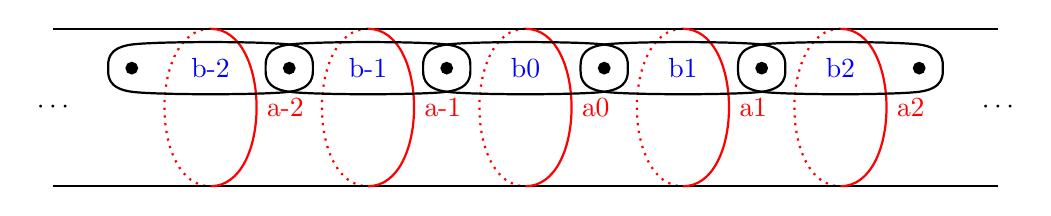
\begin{tikzpicture}[scale=2, thick]
    
    \foreach \i in {-2, -1, 0, 1, 2}
        \draw [red, dotted] (\i+0.5, 0.5) to [out=180,in=180] (\i+0.5, -0.5);
    
    \draw (3.5, 0.5) to (-2.5, 0.5);
    \draw (3.5, -0.5) to (-2.5, -0.5);
    
    \foreach \i in {-2, -1, 0, 1, 2, 3}
        \node [dot] at (\i, 0.25) {};
    
    \foreach \i in {-2, -1, 0, 1, 2}
        \draw [red] (\i+0.5, 0.5) to [out=0,in=0] node [right] {a\i} (\i+0.5, -0.5);
    
    \foreach \i in {-2, -1, 0, 1, 2} {
        \draw plot [blue, smooth cycle] coordinates {(\i-1.15+1, 0.25) (\i+0, 0.4) (\i+1, 0.4) (\i+1.15, 0.25) (\i+1, 0.1) (\i+0, 0.1)};
        \node [blue] at (\i+0.5, 0.25) {b\i};
    }
    
    \node at (3.5, 0) {$\cdots$};
    \node at (-2.5, 0) {$\cdots$};
    
\end{tikzpicture}
\end{document}
